\documentclass[10pt,aspectratio=169]{beamer}
\usetheme{metropolis}
\usepackage[T1]{fontenc}
\usepackage[utf8]{inputenc}
\usepackage{booktabs}
\usepackage{tabularx}
\usepackage{graphicx}
\usepackage{xcolor}
\usepackage{colortbl}
\usepackage{amsmath}
\usepackage{tikz}
\usetikzlibrary{arrows.meta,positioning}

\definecolor{navy}{HTML}{17324D}
\definecolor{teal}{HTML}{087E8B}
\definecolor{amber}{HTML}{C17817}
\setbeamercolor{frametitle}{bg=navy,fg=white}
\setbeamercolor{progress bar}{fg=teal}
\setbeamercolor{alerted text}{fg=amber}
\metroset{numbering=fraction,progressbar=frametitle,block=fill}
\setlength{\tabcolsep}{5pt}
\newcolumntype{Y}{>{\raggedright\arraybackslash}X}
\graphicspath{{report/slides/figures/}{outputs/task2_masks/}{outputs/task1/}}

\title{Reasoning-first Aligning two traversals of the same route}
\author{Songlin Zhang, PhD}
\date{}

\begin{document}

\maketitle

% ==================================================================
\begin{frame}{The task, in one sentence}
\begin{center}
\colorbox{teal!10}{\parbox{0.94\textwidth}{\centering\scriptsize
\textbf{We are aligning two side-camera videos recorded on the same loop route, eleven months apart, without GPS or calibration:} for every frame of the first drive, which frame of the second shows the same place, and how sure.}}
\end{center}
\footnotesize
\begin{columns}[T]
\column{0.6\textwidth}
\textbf{What I found when I first looked at the data} --- before touching any model:
\begin{enumerate}
  \item \textbf{The two drives look very different.} Dry afternoon vs rainy dusk; the second is 2.2$\times$ darker with raindrops stuck on the lens; a sideways camera changes with every lane shift.
  \item \textbf{No sensor to lean on.} No GPS, motion sensor or camera calibration anywhere in the files (checked inside the stream). Only the pictures.
  \item \textbf{Long stretches that all look the same} --- the hardest. Fences, tree tunnels: a frame looks like its neighbours, and like a spot minutes away (2.4$\times$ worse on the right camera).
  \item \textbf{Some things that look like noise turn out to be systematic}: a slight drift of the right camera's angle, which affects alignment if unhandled; lane changes; speed bumps (slide 17).
\end{enumerate}
\column{0.38\textwidth}
\vspace{-4pt}
\begin{block}{How a person solves it}
Nobody recognises a single frame of fence. A person scrubs back and forth and watches what comes \emph{before and after}: the order tells you what one picture cannot. So the algorithm should use the order too, and decide over a stretch of video.
\end{block}
\vspace{2pt}
\begin{center}
\colorbox{teal!10}{\parbox{0.96\linewidth}{\centering\footnotesize\textbf{So I framed it as a sequence alignment problem instead of independent image matching.}}}
\end{center}
\end{columns}
\end{frame}

% ==================================================================
\begin{frame}{Stage 1 \,·\, 1.1 Decode one fixed way}
\vspace{-5pt}
{\footnotesize \textbf{First, I make the videos reliable before any matching.}}
\vspace{-6pt}
\begin{center}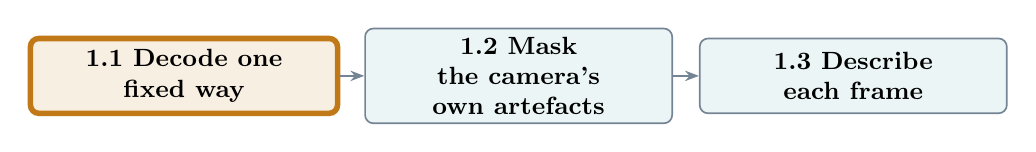
\begin{tikzpicture}[x=1cm,y=1cm]
\node[rectangle,rounded corners=3pt,draw=amber,line width=2pt,fill=amber!12,minimum width=3.9cm,minimum height=0.95cm,text width=3.60cm,align=center,font=\small\bfseries,inner sep=3pt] (s0) at (0.00,0) {1.1 Decode one\\fixed way};
\node[rectangle,rounded corners=3pt,draw=navy!60,line width=0.6pt,fill=teal!8,minimum width=3.9cm,minimum height=0.95cm,text width=3.60cm,align=center,font=\small\bfseries,inner sep=3pt] (s1) at (4.25,0) {1.2 Mask the camera's\\own artefacts};
\draw[-{Stealth[length=5pt]},navy!60,line width=0.8pt] (s0.east) -- (s1.west);
\node[rectangle,rounded corners=3pt,draw=navy!60,line width=0.6pt,fill=teal!8,minimum width=3.9cm,minimum height=0.95cm,text width=3.60cm,align=center,font=\small\bfseries,inner sep=3pt] (s2) at (8.50,0) {1.3 Describe\\each frame};
\draw[-{Stealth[length=5pt]},navy!60,line width=0.8pt] (s1.east) -- (s2.west);
\end{tikzpicture}\end{center}
\vspace{-9pt}\begin{center}\tiny \textbf{Stage 1 · Prepare the frames} $\rightarrow$ \textcolor{navy!55}{Stage 2 · Sequence matching} $\rightarrow$ \textcolor{navy!55}{Stage 3 · Geometric verification and decision}\end{center}
\vspace{-3pt}
\footnotesize\setlength{\tabcolsep}{5pt}\renewcommand{\arraystretch}{1.05}
\begin{tabularx}{\textwidth}{@{}>{\raggedright\arraybackslash}p{0.36\textwidth}>{\raggedright\arraybackslash}X@{}}
\toprule \textcolor{navy}{\textbf{Problem}} & \textcolor{navy}{\textbf{Method chosen, and why}} \\ \midrule
\textbf{Stored order $\neq$ display order} for 74.4\% of pictures (B-pyramid 0, 4, 2, 1, 3, \dots). & I fixed the decoding issue where storage order didn't match display order by \textbf{writing a small parser} that rebuilds the picture order from the stream, so frame identity is preserved. (A 1--3-frame scramble is the size of the error being measured.) \\
\addlinespace[3pt]
\textbf{No colour matrix declared}; pinning one changes 3.17\% of decoded bytes. & I \textbf{standardised colour handling} where the matrix was unspecified (BT.709 pinned, decoded from the original stream), to keep appearance consistent across tools. \\
\addlinespace[3pt]
Any of the above can \textbf{drift silently} when code or settings change. & To prevent silent drifts when configs change, I \textbf{bake the data assumptions into the cache key and add integrity checks} (24 gates: 22 pass, 2 waived on record). \\
\bottomrule\end{tabularx}
\end{frame}

% ==================================================================
\begin{frame}{Stage 1 \,·\, 1.2 Mask the camera's own artefacts}
\vspace{-5pt}
{\footnotesize \textbf{Before extracting descriptors, I mask fixed artefacts like raindrops and mirrors using temporal statistics}, with a rule insensitive to the drives' exposure difference.}
\vspace{-6pt}
\begin{center}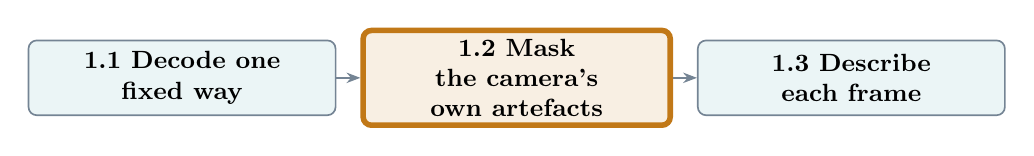
\begin{tikzpicture}[x=1cm,y=1cm]
\node[rectangle,rounded corners=3pt,draw=navy!60,line width=0.6pt,fill=teal!8,minimum width=3.9cm,minimum height=0.95cm,text width=3.60cm,align=center,font=\small\bfseries,inner sep=3pt] (s0) at (0.00,0) {1.1 Decode one\\fixed way};
\node[rectangle,rounded corners=3pt,draw=amber,line width=2pt,fill=amber!12,minimum width=3.9cm,minimum height=0.95cm,text width=3.60cm,align=center,font=\small\bfseries,inner sep=3pt] (s1) at (4.25,0) {1.2 Mask the camera's\\own artefacts};
\draw[-{Stealth[length=5pt]},navy!60,line width=0.8pt] (s0.east) -- (s1.west);
\node[rectangle,rounded corners=3pt,draw=navy!60,line width=0.6pt,fill=teal!8,minimum width=3.9cm,minimum height=0.95cm,text width=3.60cm,align=center,font=\small\bfseries,inner sep=3pt] (s2) at (8.50,0) {1.3 Describe\\each frame};
\draw[-{Stealth[length=5pt]},navy!60,line width=0.8pt] (s1.east) -- (s2.west);
\end{tikzpicture}\end{center}
\vspace{-9pt}\begin{center}\tiny \textbf{Stage 1 · Prepare the frames} $\rightarrow$ \textcolor{navy!55}{Stage 2 · Sequence matching} $\rightarrow$ \textcolor{navy!55}{Stage 3 · Geometric verification and decision}\end{center}
\vspace{-3pt}
\footnotesize\setlength{\tabcolsep}{5pt}\renewcommand{\arraystretch}{1.05}
\begin{tabularx}{\textwidth}{@{}>{\raggedright\arraybackslash}p{0.36\textwidth}>{\raggedright\arraybackslash}X@{}}
\toprule \textcolor{navy}{\textbf{Problem}} & \textcolor{navy}{\textbf{Method chosen, and why}} \\ \midrule
\textbf{Raindrops fixed on the lens} for the whole rainy drive. & \textbf{Mask from temporal statistics}: staticness $= |\nabla(\text{temporal median})| / (\text{temporal std} + 1)$ with a relative-contrast guard. Camera-attached content is exactly what stays static while the scene moves. \\
\addlinespace[3pt]
\textbf{Wing mirror and vignette} always in frame. & Same statistic, plus a \textbf{never-bright} test (temporal max $< 18\%$ of p99). Dead lens areas never get bright, whatever the scene. \\
\addlinespace[3pt]
\textbf{Rainy drive 2.2$\times$ darker}; segmenters (ADE20K) have no class for any of this. & No learned model; the ratio is near scale-free, computed per drive at $360\times270$ over every 8th frame, versioned. Same rule on both drives, no label consumed. \\
\bottomrule\end{tabularx}
\end{frame}

% ==================================================================
\begin{frame}{Stage 1 \,·\, 1.2 Mask the camera's own artefacts (in pictures)}
\vspace{-5pt}
\begin{center}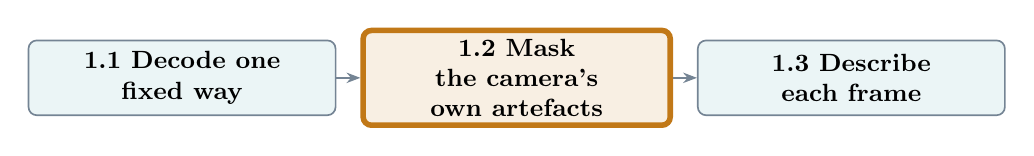
\begin{tikzpicture}[x=1cm,y=1cm]
\node[rectangle,rounded corners=3pt,draw=navy!60,line width=0.6pt,fill=teal!8,minimum width=3.9cm,minimum height=0.95cm,text width=3.60cm,align=center,font=\small\bfseries,inner sep=3pt] (s0) at (0.00,0) {1.1 Decode one\\fixed way};
\node[rectangle,rounded corners=3pt,draw=amber,line width=2pt,fill=amber!12,minimum width=3.9cm,minimum height=0.95cm,text width=3.60cm,align=center,font=\small\bfseries,inner sep=3pt] (s1) at (4.25,0) {1.2 Mask the camera's\\own artefacts};
\draw[-{Stealth[length=5pt]},navy!60,line width=0.8pt] (s0.east) -- (s1.west);
\node[rectangle,rounded corners=3pt,draw=navy!60,line width=0.6pt,fill=teal!8,minimum width=3.9cm,minimum height=0.95cm,text width=3.60cm,align=center,font=\small\bfseries,inner sep=3pt] (s2) at (8.50,0) {1.3 Describe\\each frame};
\draw[-{Stealth[length=5pt]},navy!60,line width=0.8pt] (s1.east) -- (s2.west);
\end{tikzpicture}\end{center}
\vspace{-9pt}\begin{center}\tiny \textbf{Stage 1 · Prepare the frames} $\rightarrow$ \textcolor{navy!55}{Stage 2 · Sequence matching} $\rightarrow$ \textcolor{navy!55}{Stage 3 · Geometric verification and decision}\end{center}
\vspace{-3pt}
\begin{columns}[T]\column{0.5\textwidth}\centering
\includegraphics[width=\linewidth,height=2.9cm,keepaspectratio]{sd_maps.png}\\[-1pt]{\scriptsize How much each pixel changed over the whole drive. The drops, the mirror and the dark corners never move, which is why a temporal statistic finds them.}\column{0.48\textwidth}\centering
\includegraphics[width=0.48\linewidth]{runA_cam0_mask_overlay.png}\hspace{0.02\linewidth}
\includegraphics[width=0.48\linewidth]{runB_cam0_mask_overlay.png}\\[-1pt]{\scriptsize The resulting mask on the dry drive (left) and the rainy drive (right): red is camera-attached, blue too dark to use. Same rule; only the rainy drive grows drops.}\end{columns}
\end{frame}

\begin{frame}{Stage 1 \,·\, 1.2 Mask the camera's own artefacts: first attempt}
\vspace{-5pt}
\begin{center}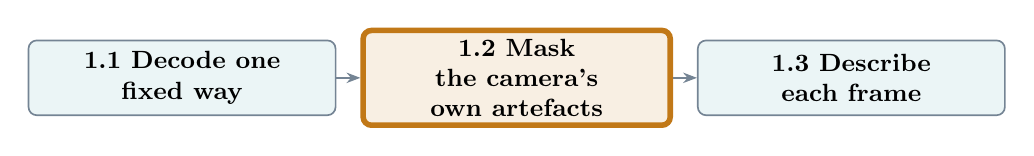
\begin{tikzpicture}[x=1cm,y=1cm]
\node[rectangle,rounded corners=3pt,draw=navy!60,line width=0.6pt,fill=teal!8,minimum width=3.9cm,minimum height=0.95cm,text width=3.60cm,align=center,font=\small\bfseries,inner sep=3pt] (s0) at (0.00,0) {1.1 Decode one\\fixed way};
\node[rectangle,rounded corners=3pt,draw=amber,line width=2pt,fill=amber!12,minimum width=3.9cm,minimum height=0.95cm,text width=3.60cm,align=center,font=\small\bfseries,inner sep=3pt] (s1) at (4.25,0) {1.2 Mask the camera's\\own artefacts};
\draw[-{Stealth[length=5pt]},navy!60,line width=0.8pt] (s0.east) -- (s1.west);
\node[rectangle,rounded corners=3pt,draw=navy!60,line width=0.6pt,fill=teal!8,minimum width=3.9cm,minimum height=0.95cm,text width=3.60cm,align=center,font=\small\bfseries,inner sep=3pt] (s2) at (8.50,0) {1.3 Describe\\each frame};
\draw[-{Stealth[length=5pt]},navy!60,line width=0.8pt] (s1.east) -- (s2.west);
\end{tikzpicture}\end{center}
\vspace{-9pt}\begin{center}\tiny \textbf{Stage 1 · Prepare the frames} $\rightarrow$ \textcolor{navy!55}{Stage 2 · Sequence matching} $\rightarrow$ \textcolor{navy!55}{Stage 3 · Geometric verification and decision}\end{center}
\vspace{2pt}
\begin{center}
\colorbox{teal!10}{\parbox{0.94\textwidth}{\small \textbf{I first tried SegFormer, but it doesn't cover raindrops, mirrors or dark vignetting --- which are our main artefacts --- so I switched to a temporal-statistics mask.}}}
\end{center}
\vspace{2pt}
\scriptsize
\begin{itemize}
  \item Note: on the 8-pair development set SegFormer removed one false accept (3 $\to$ 2) but cut coarse retrieval recall@5 from 0.71 to 0.57. The temporal mask finds the rain where it is: right camera 1.2\% (dry) $\to$ 9.9\% (rainy).
  \item Honest attribution: the mask was rebuilt together with the decode and the dense path, so its effect alone is not isolated in a held-out test.
\end{itemize}
\end{frame}

% ==================================================================
\begin{frame}{Stage 1 \,·\, 1.3 Describe each frame}
\vspace{-5pt}
\begin{center}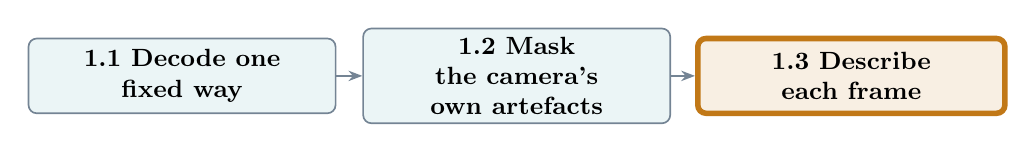
\begin{tikzpicture}[x=1cm,y=1cm]
\node[rectangle,rounded corners=3pt,draw=navy!60,line width=0.6pt,fill=teal!8,minimum width=3.9cm,minimum height=0.95cm,text width=3.60cm,align=center,font=\small\bfseries,inner sep=3pt] (s0) at (0.00,0) {1.1 Decode one\\fixed way};
\node[rectangle,rounded corners=3pt,draw=navy!60,line width=0.6pt,fill=teal!8,minimum width=3.9cm,minimum height=0.95cm,text width=3.60cm,align=center,font=\small\bfseries,inner sep=3pt] (s1) at (4.25,0) {1.2 Mask the camera's\\own artefacts};
\draw[-{Stealth[length=5pt]},navy!60,line width=0.8pt] (s0.east) -- (s1.west);
\node[rectangle,rounded corners=3pt,draw=amber,line width=2pt,fill=amber!12,minimum width=3.9cm,minimum height=0.95cm,text width=3.60cm,align=center,font=\small\bfseries,inner sep=3pt] (s2) at (8.50,0) {1.3 Describe\\each frame};
\draw[-{Stealth[length=5pt]},navy!60,line width=0.8pt] (s1.east) -- (s2.west);
\end{tikzpicture}\end{center}
\vspace{-9pt}\begin{center}\tiny \textbf{Stage 1 · Prepare the frames} $\rightarrow$ \textcolor{navy!55}{Stage 2 · Sequence matching} $\rightarrow$ \textcolor{navy!55}{Stage 3 · Geometric verification and decision}\end{center}
\vspace{-3pt}
\footnotesize\setlength{\tabcolsep}{5pt}\renewcommand{\arraystretch}{1.05}
\begin{tabularx}{\textwidth}{@{}>{\raggedright\arraybackslash}p{0.36\textwidth}>{\raggedright\arraybackslash}X@{}}
\toprule \textcolor{navy}{\textbf{Problem}} & \textcolor{navy}{\textbf{Method chosen, and why}} \\ \midrule
\textbf{Eleven months apart}, dry afternoon against rainy dusk. & Because the runs are months apart, I start with \textbf{frozen DINOv2 patch features and cosine similarity} to get robust coarse matches under lighting change (ViT-S/14 at $448\times336$, nothing fine-tuned). \\
\addlinespace[3pt]
\textbf{No labels to train with}: the only labels that exist are the blind test set. & \textbf{Nothing fine-tuned}. Training would either need labels I do not have or spend the test. \\
\addlinespace[3pt]
Droplets and the mirror would \textbf{bias a whole-image descriptor}. & \textbf{Masked mean pooling} over reliable patches only. Remove the bias rather than hope the network ignores it. (An unsupervised VLAD pooling over the same tokens is evaluated later as a variant.) \\
\bottomrule\end{tabularx}
\end{frame}

% ==================================================================
\begin{frame}{Stage 2 \,·\, 2.1 Compare with the whole other drive}
\vspace{-5pt}
\vspace{-2pt}{\footnotesize The frames can now be trusted. Stage 2 is \textbf{sequence matching}, coarse to fine: it finds roughly \emph{where} each frame belongs. This page answers \emph{where do I search?}, the next \emph{how do I find the path?}}
\vspace{-6pt}
\begin{center}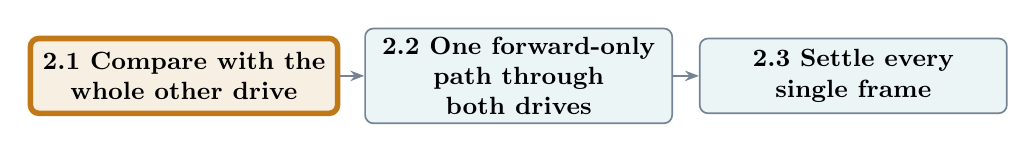
\begin{tikzpicture}[x=1cm,y=1cm]
\node[rectangle,rounded corners=3pt,draw=amber,line width=2pt,fill=amber!12,minimum width=3.9cm,minimum height=0.95cm,text width=3.60cm,align=center,font=\small\bfseries,inner sep=3pt] (s0) at (0.00,0) {2.1 Compare with the\\whole other drive};
\node[rectangle,rounded corners=3pt,draw=navy!60,line width=0.6pt,fill=teal!8,minimum width=3.9cm,minimum height=0.95cm,text width=3.60cm,align=center,font=\small\bfseries,inner sep=3pt] (s1) at (4.25,0) {2.2 One forward-only\\path through both drives};
\draw[-{Stealth[length=5pt]},navy!60,line width=0.8pt] (s0.east) -- (s1.west);
\node[rectangle,rounded corners=3pt,draw=navy!60,line width=0.6pt,fill=teal!8,minimum width=3.9cm,minimum height=0.95cm,text width=3.60cm,align=center,font=\small\bfseries,inner sep=3pt] (s2) at (8.50,0) {2.3 Settle every\\single frame};
\draw[-{Stealth[length=5pt]},navy!60,line width=0.8pt] (s1.east) -- (s2.west);
\end{tikzpicture}\end{center}
\vspace{-9pt}\begin{center}\tiny \textcolor{navy!55}{Stage 1 · Prepare the frames} $\rightarrow$ \textbf{Stage 2 · Sequence matching} $\rightarrow$ \textcolor{navy!55}{Stage 3 · Geometric verification and decision}\end{center}
\vspace{-3pt}
\footnotesize\setlength{\tabcolsep}{5pt}\renewcommand{\arraystretch}{1.05}
\begin{tabularx}{\textwidth}{@{}>{\raggedright\arraybackslash}p{0.36\textwidth}>{\raggedright\arraybackslash}X@{}}
\toprule \textcolor{navy}{\textbf{Problem}} & \textcolor{navy}{\textbf{Method chosen, and why}} \\ \midrule
At full resolution, \textbf{matching every frame is too expensive}. & So I start with a \textbf{coarse pass}, sampling every fourth frame of both drives. \\
\addlinespace[3pt]
\textbf{Where do I search?} Look-alike places are sometimes hundreds of frames apart, and the time offset between the drives drifts by around 12 seconds. & A local search band is risky because of that drift, so I compute a \textbf{full similarity matrix} over the whole other drive and keep it cheap by subsampling. \\
\bottomrule\end{tabularx}
\end{frame}

% ==================================================================
\begin{frame}{Stage 2 \,·\, 2.2 One forward-only path}
\vspace{-5pt}
\begin{center}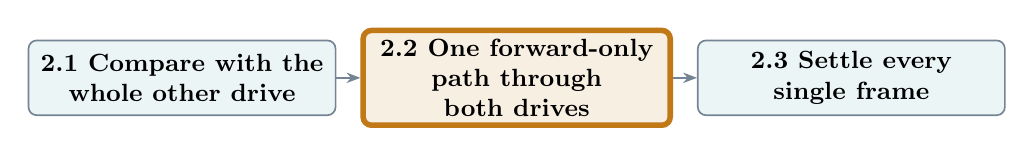
\begin{tikzpicture}[x=1cm,y=1cm]
\node[rectangle,rounded corners=3pt,draw=navy!60,line width=0.6pt,fill=teal!8,minimum width=3.9cm,minimum height=0.95cm,text width=3.60cm,align=center,font=\small\bfseries,inner sep=3pt] (s0) at (0.00,0) {2.1 Compare with the\\whole other drive};
\node[rectangle,rounded corners=3pt,draw=amber,line width=2pt,fill=amber!12,minimum width=3.9cm,minimum height=0.95cm,text width=3.60cm,align=center,font=\small\bfseries,inner sep=3pt] (s1) at (4.25,0) {2.2 One forward-only\\path through both drives};
\draw[-{Stealth[length=5pt]},navy!60,line width=0.8pt] (s0.east) -- (s1.west);
\node[rectangle,rounded corners=3pt,draw=navy!60,line width=0.6pt,fill=teal!8,minimum width=3.9cm,minimum height=0.95cm,text width=3.60cm,align=center,font=\small\bfseries,inner sep=3pt] (s2) at (8.50,0) {2.3 Settle every\\single frame};
\draw[-{Stealth[length=5pt]},navy!60,line width=0.8pt] (s1.east) -- (s2.west);
\end{tikzpicture}\end{center}
\vspace{-9pt}\begin{center}\tiny \textcolor{navy!55}{Stage 1 · Prepare the frames} $\rightarrow$ \textbf{Stage 2 · Sequence matching} $\rightarrow$ \textcolor{navy!55}{Stage 3 · Geometric verification and decision}\end{center}
\vspace{-3pt}
\footnotesize\setlength{\tabcolsep}{5pt}\renewcommand{\arraystretch}{1.05}
\begin{tabularx}{\textwidth}{@{}>{\raggedright\arraybackslash}p{0.36\textwidth}>{\raggedright\arraybackslash}X@{}}
\toprule \textcolor{navy}{\textbf{Problem}} & \textcolor{navy}{\textbf{Method chosen, and why}} \\ \midrule
\textbf{How do I find the path?} In a fence corridor a single frame carries no identity; a person uses the order of events. & \textbf{Dynamic time warping}: one path through the similarity matrix that can only move forward. Order is the constraint a person actually uses. \\
\addlinespace[3pt]
The two drives were \textbf{recorded at different speeds}, and the ratio changes along the route. & I \textbf{let the slope vary within measured limits}: the bounds come from the drift I measured, not from an assumption. \\
\addlinespace[3pt]
The route is a \textbf{loop}: departure and arrival look alike, so a naive search wraps across the seam. & Departure and arrival are treated as \textbf{distinct occurrences}: no wrap, no interpolation across the seam. \\
\bottomrule\end{tabularx}
\vspace{2pt}
{\tiny\textcolor{navy!60}{Note: step set $\{(1,1),(1,2),(2,1),(1,3),(3,1),(2,2)\}$, slope penalty 0.035, skip penalty 0.008, local slope in $[0.2, 2.0]$.}}
\end{frame}

% ==================================================================
\begin{frame}{Stage 2 \,·\, 2.2 One forward-only path (in pictures)}
\vspace{-5pt}
\begin{center}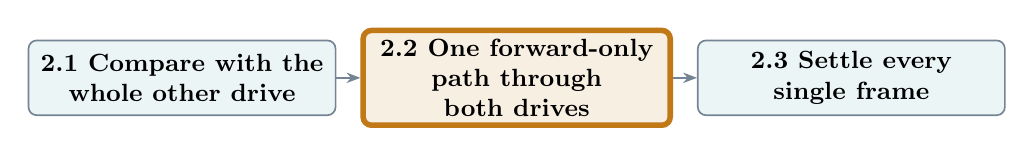
\begin{tikzpicture}[x=1cm,y=1cm]
\node[rectangle,rounded corners=3pt,draw=navy!60,line width=0.6pt,fill=teal!8,minimum width=3.9cm,minimum height=0.95cm,text width=3.60cm,align=center,font=\small\bfseries,inner sep=3pt] (s0) at (0.00,0) {2.1 Compare with the\\whole other drive};
\node[rectangle,rounded corners=3pt,draw=amber,line width=2pt,fill=amber!12,minimum width=3.9cm,minimum height=0.95cm,text width=3.60cm,align=center,font=\small\bfseries,inner sep=3pt] (s1) at (4.25,0) {2.2 One forward-only\\path through both drives};
\draw[-{Stealth[length=5pt]},navy!60,line width=0.8pt] (s0.east) -- (s1.west);
\node[rectangle,rounded corners=3pt,draw=navy!60,line width=0.6pt,fill=teal!8,minimum width=3.9cm,minimum height=0.95cm,text width=3.60cm,align=center,font=\small\bfseries,inner sep=3pt] (s2) at (8.50,0) {2.3 Settle every\\single frame};
\draw[-{Stealth[length=5pt]},navy!60,line width=0.8pt] (s1.east) -- (s2.west);
\end{tikzpicture}\end{center}
\vspace{-9pt}\begin{center}\tiny \textcolor{navy!55}{Stage 1 · Prepare the frames} $\rightarrow$ \textbf{Stage 2 · Sequence matching} $\rightarrow$ \textcolor{navy!55}{Stage 3 · Geometric verification and decision}\end{center}
\vspace{-3pt}
\begin{columns}[T]\column{0.5\textwidth}\centering
\includegraphics[width=0.9\linewidth,height=1.6cm,keepaspectratio]{loop_first_last_cam0.png}\\[-1pt]{\scriptsize First and last frames: the car returns to the same bay, same heading. The route is a loop, so its two ends alias.}\\[3pt]
\includegraphics[width=0.9\linewidth,height=1.5cm,keepaspectratio]{cam0_loop_closure_comparison.png}\\[-1pt]{\scriptsize Leaving and returning: the same place at both ends. The path may not jump across this seam.}\column{0.48\textwidth}\begin{center}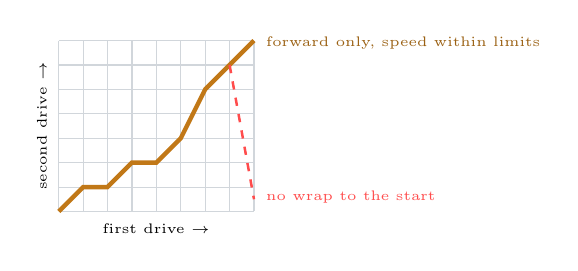
\begin{tikzpicture}[x=0.31cm,y=0.31cm]
\draw[step=1,navy!20,thin] (0,0) grid (8,7);
\node[font=\tiny,anchor=north] at (4,-0.1) {first drive $\rightarrow$};
\node[font=\tiny,rotate=90,anchor=south] at (-0.1,3.5) {second drive $\rightarrow$};
\draw[amber,line width=1.6pt] (0,0) -- (1,1) -- (2,1) -- (3,2) -- (4,2) -- (5,3) -- (6,5) -- (7,6) -- (8,7);
\draw[red!70,dashed,line width=0.9pt] (7,6) -- (8,0.5);
\node[font=\tiny,red!70,anchor=west] at (8.1,0.6) {no wrap to the start};
\node[font=\tiny,amber!80!black,anchor=west] at (8.1,6.9) {forward only, speed within limits};
\end{tikzpicture}\end{center}{\scriptsize One path through the similarity grid: it may only move right or up, at a bounded slope, and never back to the start.}\end{columns}
\end{frame}

% ==================================================================
\begin{frame}{Stage 2 \,·\, 2.3 Settle every single frame}
\vspace{-5pt}
\begin{center}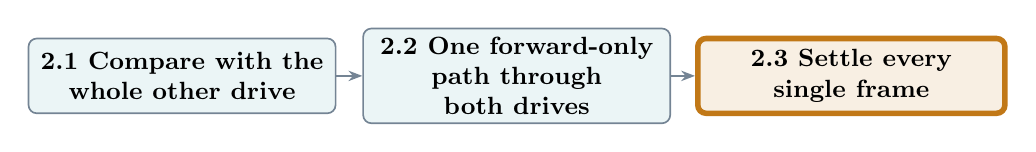
\begin{tikzpicture}[x=1cm,y=1cm]
\node[rectangle,rounded corners=3pt,draw=navy!60,line width=0.6pt,fill=teal!8,minimum width=3.9cm,minimum height=0.95cm,text width=3.60cm,align=center,font=\small\bfseries,inner sep=3pt] (s0) at (0.00,0) {2.1 Compare with the\\whole other drive};
\node[rectangle,rounded corners=3pt,draw=navy!60,line width=0.6pt,fill=teal!8,minimum width=3.9cm,minimum height=0.95cm,text width=3.60cm,align=center,font=\small\bfseries,inner sep=3pt] (s1) at (4.25,0) {2.2 One forward-only\\path through both drives};
\draw[-{Stealth[length=5pt]},navy!60,line width=0.8pt] (s0.east) -- (s1.west);
\node[rectangle,rounded corners=3pt,draw=amber,line width=2pt,fill=amber!12,minimum width=3.9cm,minimum height=0.95cm,text width=3.60cm,align=center,font=\small\bfseries,inner sep=3pt] (s2) at (8.50,0) {2.3 Settle every\\single frame};
\draw[-{Stealth[length=5pt]},navy!60,line width=0.8pt] (s1.east) -- (s2.west);
\end{tikzpicture}\end{center}
\vspace{-9pt}\begin{center}\tiny \textcolor{navy!55}{Stage 1 · Prepare the frames} $\rightarrow$ \textbf{Stage 2 · Sequence matching} $\rightarrow$ \textcolor{navy!55}{Stage 3 · Geometric verification and decision}\end{center}
\vspace{-3pt}
\footnotesize\setlength{\tabcolsep}{5pt}\renewcommand{\arraystretch}{1.05}
\begin{tabularx}{\textwidth}{@{}>{\raggedright\arraybackslash}p{0.36\textwidth}>{\raggedright\arraybackslash}X@{}}
\toprule \textcolor{navy}{\textbf{Problem}} & \textcolor{navy}{\textbf{Method chosen, and why}} \\ \midrule
Stride 4 leaves a \textbf{$\pm2$-frame ambiguity}; a consumer needs the exact frame. & \textbf{Full-cadence refinement}: for every frame, argmax of a local structure score within $\pm8$ of the interpolated coarse path. The coarse path already fixes the neighbourhood, so this is cheap. \\
\addlinespace[3pt]
The result must \textbf{stay in sequence order}. & Refinement runs under a \textbf{non-decreasing floor}. \\
\addlinespace[3pt]
\textbf{A defect}: this stage has \textbf{no speed (slope) prior}. Where the local score is flat, the optimiser runs to the window edge, producing implausible jumps --- at high confidence. & I \textbf{reported the limitation} as it is. After the freeze I built a \textbf{Viterbi version with a slope prior} that avoids the jumps by construction; because it came after the freeze, it is reference evidence, not the submission. \\
\bottomrule\end{tabularx}
\end{frame}

% ==================================================================
\begin{frame}{Stage 2 \,·\, 2.3 Settle every single frame (in pictures)}
\vspace{-5pt}
\begin{center}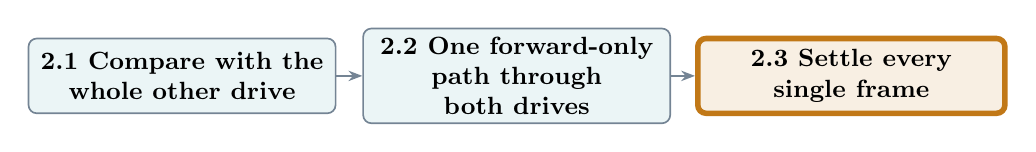
\begin{tikzpicture}[x=1cm,y=1cm]
\node[rectangle,rounded corners=3pt,draw=navy!60,line width=0.6pt,fill=teal!8,minimum width=3.9cm,minimum height=0.95cm,text width=3.60cm,align=center,font=\small\bfseries,inner sep=3pt] (s0) at (0.00,0) {2.1 Compare with the\\whole other drive};
\node[rectangle,rounded corners=3pt,draw=navy!60,line width=0.6pt,fill=teal!8,minimum width=3.9cm,minimum height=0.95cm,text width=3.60cm,align=center,font=\small\bfseries,inner sep=3pt] (s1) at (4.25,0) {2.2 One forward-only\\path through both drives};
\draw[-{Stealth[length=5pt]},navy!60,line width=0.8pt] (s0.east) -- (s1.west);
\node[rectangle,rounded corners=3pt,draw=amber,line width=2pt,fill=amber!12,minimum width=3.9cm,minimum height=0.95cm,text width=3.60cm,align=center,font=\small\bfseries,inner sep=3pt] (s2) at (8.50,0) {2.3 Settle every\\single frame};
\draw[-{Stealth[length=5pt]},navy!60,line width=0.8pt] (s1.east) -- (s2.west);
\end{tikzpicture}\end{center}
\vspace{-9pt}\begin{center}\tiny \textcolor{navy!55}{Stage 1 · Prepare the frames} $\rightarrow$ \textbf{Stage 2 · Sequence matching} $\rightarrow$ \textcolor{navy!55}{Stage 3 · Geometric verification and decision}\end{center}
\vspace{-3pt}
\begin{columns}[T]\column{0.6\textwidth}\centering
\includegraphics[width=\linewidth,height=4.0cm,keepaspectratio]{kink_A905.png}\column{0.38\textwidth}\footnotesize\vspace{6pt}What this stage's defect looks like: frame 905 of the first drive mapped to frame 802 of the second at top confidence --- two different houses. Found by rendering the aligned videos side by side with guide lines, the same habit as looking at the data in the first place.\end{columns}
\end{frame}

% ==================================================================
\begin{frame}{Stage 3 \,·\, 3.1 Uniqueness check}
\vspace{-5pt}
\vspace{-2pt}{\footnotesize Stage 2 says roughly where I am. Stage 3 checks that the match is unique, confirms the exact frame \textbf{geometrically on the pixels}, and decides whether to answer at all.}
\vspace{-6pt}
\begin{center}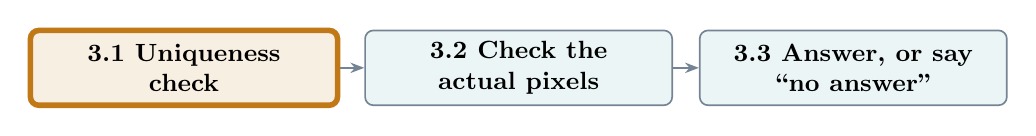
\begin{tikzpicture}[x=1cm,y=1cm]
\node[rectangle,rounded corners=3pt,draw=amber,line width=2pt,fill=amber!12,minimum width=3.9cm,minimum height=0.95cm,text width=3.60cm,align=center,font=\small\bfseries,inner sep=3pt] (s0) at (0.00,0) {3.1 Uniqueness\\check};
\node[rectangle,rounded corners=3pt,draw=navy!60,line width=0.6pt,fill=teal!8,minimum width=3.9cm,minimum height=0.95cm,text width=3.60cm,align=center,font=\small\bfseries,inner sep=3pt] (s1) at (4.25,0) {3.2 Check the\\actual pixels};
\draw[-{Stealth[length=5pt]},navy!60,line width=0.8pt] (s0.east) -- (s1.west);
\node[rectangle,rounded corners=3pt,draw=navy!60,line width=0.6pt,fill=teal!8,minimum width=3.9cm,minimum height=0.95cm,text width=3.60cm,align=center,font=\small\bfseries,inner sep=3pt] (s2) at (8.50,0) {3.3 Answer, or say\\``no answer''};
\draw[-{Stealth[length=5pt]},navy!60,line width=0.8pt] (s1.east) -- (s2.west);
\end{tikzpicture}\end{center}
\vspace{-9pt}\begin{center}\tiny \textcolor{navy!55}{Stage 1 · Prepare the frames} $\rightarrow$ \textcolor{navy!55}{Stage 2 · Sequence matching} $\rightarrow$ \textbf{Stage 3 · Geometric verification and decision}\end{center}
\vspace{-3pt}
\footnotesize\setlength{\tabcolsep}{5pt}\renewcommand{\arraystretch}{1.05}
\begin{tabularx}{\textwidth}{@{}>{\raggedright\arraybackslash}p{0.36\textwidth}>{\raggedright\arraybackslash}X@{}}
\toprule \textcolor{navy}{\textbf{Problem}} & \textcolor{navy}{\textbf{Method chosen, and why}} \\ \midrule
Some corridors and tree stretches look \textbf{almost identical}, so a single frame is easily misjudged. & \textbf{Multi-scale sequence uniqueness}: I compare the best match against the second-best, to make sure this stretch is genuinely distinctive. \\
\addlinespace[3pt]
Repeated scenery comes at \textbf{different lengths} --- short awnings, long tree tunnels. & I check for repeated segments at \textbf{several window scales}, using windows of different radii (2 / 5 / 10 / 20 nodes) to confirm uniqueness. \\
\addlinespace[3pt]
What should \textbf{confidence} mean here? & Confidence reflects \textbf{uniqueness, not strength}: how big the gap is between the best and the second-best match, not how high the score is. That gap assigns the \emph{strong} and \emph{sequence-supported} tiers. \\
\bottomrule\end{tabularx}
\end{frame}

% ==================================================================
\begin{frame}{Stage 3 \,·\, 3.2 Check the actual pixels}
\vspace{-5pt}
\begin{center}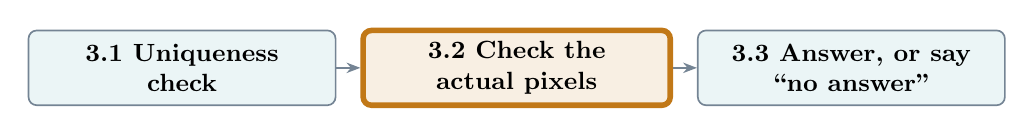
\begin{tikzpicture}[x=1cm,y=1cm]
\node[rectangle,rounded corners=3pt,draw=navy!60,line width=0.6pt,fill=teal!8,minimum width=3.9cm,minimum height=0.95cm,text width=3.60cm,align=center,font=\small\bfseries,inner sep=3pt] (s0) at (0.00,0) {3.1 Uniqueness\\check};
\node[rectangle,rounded corners=3pt,draw=amber,line width=2pt,fill=amber!12,minimum width=3.9cm,minimum height=0.95cm,text width=3.60cm,align=center,font=\small\bfseries,inner sep=3pt] (s1) at (4.25,0) {3.2 Check the\\actual pixels};
\draw[-{Stealth[length=5pt]},navy!60,line width=0.8pt] (s0.east) -- (s1.west);
\node[rectangle,rounded corners=3pt,draw=navy!60,line width=0.6pt,fill=teal!8,minimum width=3.9cm,minimum height=0.95cm,text width=3.60cm,align=center,font=\small\bfseries,inner sep=3pt] (s2) at (8.50,0) {3.3 Answer, or say\\``no answer''};
\draw[-{Stealth[length=5pt]},navy!60,line width=0.8pt] (s1.east) -- (s2.west);
\end{tikzpicture}\end{center}
\vspace{-9pt}\begin{center}\tiny \textcolor{navy!55}{Stage 1 · Prepare the frames} $\rightarrow$ \textcolor{navy!55}{Stage 2 · Sequence matching} $\rightarrow$ \textbf{Stage 3 · Geometric verification and decision}\end{center}
\vspace{-3pt}
\footnotesize\setlength{\tabcolsep}{5pt}\renewcommand{\arraystretch}{1.05}
\begin{tabularx}{\textwidth}{@{}>{\raggedright\arraybackslash}p{0.36\textwidth}>{\raggedright\arraybackslash}X@{}}
\toprule \textcolor{navy}{\textbf{Problem}} & \textcolor{navy}{\textbf{Method chosen, and why}} \\ \midrule
Sequence order says roughly \emph{where} you are, but foliage and fences still produce \textbf{false matches} with many raw correspondences. & \textbf{Geometric verification} to filter false matches: RootSIFT + ratio test + RANSAC, a pixel-level check on the masked images. \\
\addlinespace[3pt]
A \textbf{single textured patch} (a tree crown, a fence panel) can mislead the check on its own. & I require \textbf{support across several grid cells} ($4\times3$), so one patch cannot carry the verification. \\
\addlinespace[3pt]
\textbf{Which image size} to run it at? & $896\times672$, chosen by a \textbf{resolution comparison} (next page) as the best balance between reliability and cost: at full size the share of consistent matches drops. \\
\bottomrule\end{tabularx}
\end{frame}

% ==================================================================
\begin{frame}{Stage 3 \,·\, 3.2 Check the actual pixels (the resolution study)}
\vspace{-5pt}
\begin{center}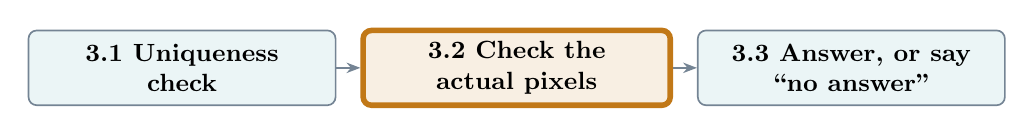
\begin{tikzpicture}[x=1cm,y=1cm]
\node[rectangle,rounded corners=3pt,draw=navy!60,line width=0.6pt,fill=teal!8,minimum width=3.9cm,minimum height=0.95cm,text width=3.60cm,align=center,font=\small\bfseries,inner sep=3pt] (s0) at (0.00,0) {3.1 Uniqueness\\check};
\node[rectangle,rounded corners=3pt,draw=amber,line width=2pt,fill=amber!12,minimum width=3.9cm,minimum height=0.95cm,text width=3.60cm,align=center,font=\small\bfseries,inner sep=3pt] (s1) at (4.25,0) {3.2 Check the\\actual pixels};
\draw[-{Stealth[length=5pt]},navy!60,line width=0.8pt] (s0.east) -- (s1.west);
\node[rectangle,rounded corners=3pt,draw=navy!60,line width=0.6pt,fill=teal!8,minimum width=3.9cm,minimum height=0.95cm,text width=3.60cm,align=center,font=\small\bfseries,inner sep=3pt] (s2) at (8.50,0) {3.3 Answer, or say\\``no answer''};
\draw[-{Stealth[length=5pt]},navy!60,line width=0.8pt] (s1.east) -- (s2.west);
\end{tikzpicture}\end{center}
\vspace{-9pt}\begin{center}\tiny \textcolor{navy!55}{Stage 1 · Prepare the frames} $\rightarrow$ \textcolor{navy!55}{Stage 2 · Sequence matching} $\rightarrow$ \textbf{Stage 3 · Geometric verification and decision}\end{center}
\vspace{-3pt}
\begin{columns}[T]\column{0.5\textwidth}\centering\scriptsize\setlength{\tabcolsep}{4pt}\textbf{left camera}\\[2pt]\begin{tabular}{lrrr}\toprule Raster & Matches & Inlier ratio & Passing \\\midrule
$448\times336$ & 22 & 0.8108 & 2/6 \\
$640\times480$ & 31 & 0.6957 & 4/6 \\
$896\times672$ & 48 & 0.6052 & 6/6 \\
$1440\times1080$ & 85 & 0.3859 & 4/6 \\
\bottomrule\end{tabular}\column{0.5\textwidth}\centering\scriptsize\setlength{\tabcolsep}{4pt}\textbf{right camera}\\[2pt]\begin{tabular}{lrrr}\toprule Raster & Matches & Inlier ratio & Passing \\\midrule
$448\times336$ & 12 & 0.7076 & 1/6 \\
$640\times480$ & 21 & 0.622 & 1/6 \\
$896\times672$ & 40 & 0.4629 & 5/6 \\
$1440\times1080$ & 86 & 0.3283 & 2/6 \\
\bottomrule\end{tabular}\end{columns}
\vspace{2pt}{\scriptsize Development pairs only. Passing peaks at $896\times672$ and falls at native, where leaf texture inflates the match count while the inlier ratio collapses.}
\end{frame}

% ==================================================================
\begin{frame}{Stage 3 \,·\, 3.3 Answer, or say ``no answer''}
\vspace{-5pt}
\begin{center}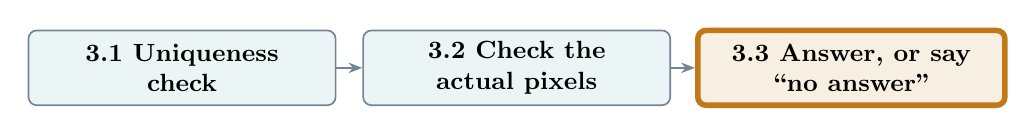
\begin{tikzpicture}[x=1cm,y=1cm]
\node[rectangle,rounded corners=3pt,draw=navy!60,line width=0.6pt,fill=teal!8,minimum width=3.9cm,minimum height=0.95cm,text width=3.60cm,align=center,font=\small\bfseries,inner sep=3pt] (s0) at (0.00,0) {3.1 Uniqueness\\check};
\node[rectangle,rounded corners=3pt,draw=navy!60,line width=0.6pt,fill=teal!8,minimum width=3.9cm,minimum height=0.95cm,text width=3.60cm,align=center,font=\small\bfseries,inner sep=3pt] (s1) at (4.25,0) {3.2 Check the\\actual pixels};
\draw[-{Stealth[length=5pt]},navy!60,line width=0.8pt] (s0.east) -- (s1.west);
\node[rectangle,rounded corners=3pt,draw=amber,line width=2pt,fill=amber!12,minimum width=3.9cm,minimum height=0.95cm,text width=3.60cm,align=center,font=\small\bfseries,inner sep=3pt] (s2) at (8.50,0) {3.3 Answer, or say\\``no answer''};
\draw[-{Stealth[length=5pt]},navy!60,line width=0.8pt] (s1.east) -- (s2.west);
\end{tikzpicture}\end{center}
\vspace{-9pt}\begin{center}\tiny \textcolor{navy!55}{Stage 1 · Prepare the frames} $\rightarrow$ \textcolor{navy!55}{Stage 2 · Sequence matching} $\rightarrow$ \textbf{Stage 3 · Geometric verification and decision}\end{center}
\vspace{-3pt}
\footnotesize\setlength{\tabcolsep}{5pt}\renewcommand{\arraystretch}{1.05}
\begin{tabularx}{\textwidth}{@{}>{\raggedright\arraybackslash}p{0.36\textwidth}>{\raggedright\arraybackslash}X@{}}
\toprule \textcolor{navy}{\textbf{Problem}} & \textcolor{navy}{\textbf{Method chosen, and why}} \\ \midrule
After uniqueness and geometry, the system must \textbf{decide whether to give a match at all}. Some frames should have no answer: blocked views, very dark stretches, no corresponding segment. & The output carries an \textbf{explicit type}: accepted (strong), accepted (sequence-supported), geometry failed, loop ambiguous, out of route, idle segment --- each refusal with a clear reason. An empty partner means \emph{no answer under this method}. \\
\addlinespace[3pt]
A \textbf{wrong answer becomes ground truth} downstream; choosing not to answer only costs coverage. & So I prefer \textbf{no answer over a confident wrong one}, and an empty row is never converted into a negative label. \\
\addlinespace[3pt]
What is the \textbf{confidence} value? & A \textbf{ranking, not a calibrated probability}. I separately implemented an HMM with a null state to get calibrated posteriors; that is reported after the freeze and is not part of the submitted method. \\
\bottomrule\end{tabularx}
\end{frame}

% ==================================================================
\begin{frame}{Stage 3 \,·\, 3.3 Answer, or say ``no answer'' (in pictures)}
\vspace{-5pt}
\begin{center}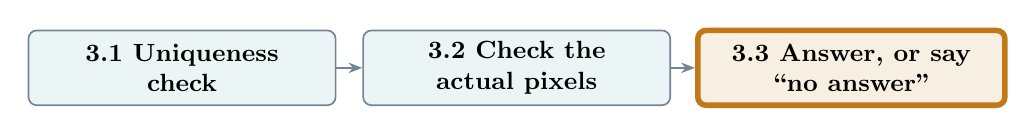
\begin{tikzpicture}[x=1cm,y=1cm]
\node[rectangle,rounded corners=3pt,draw=navy!60,line width=0.6pt,fill=teal!8,minimum width=3.9cm,minimum height=0.95cm,text width=3.60cm,align=center,font=\small\bfseries,inner sep=3pt] (s0) at (0.00,0) {3.1 Uniqueness\\check};
\node[rectangle,rounded corners=3pt,draw=navy!60,line width=0.6pt,fill=teal!8,minimum width=3.9cm,minimum height=0.95cm,text width=3.60cm,align=center,font=\small\bfseries,inner sep=3pt] (s1) at (4.25,0) {3.2 Check the\\actual pixels};
\draw[-{Stealth[length=5pt]},navy!60,line width=0.8pt] (s0.east) -- (s1.west);
\node[rectangle,rounded corners=3pt,draw=amber,line width=2pt,fill=amber!12,minimum width=3.9cm,minimum height=0.95cm,text width=3.60cm,align=center,font=\small\bfseries,inner sep=3pt] (s2) at (8.50,0) {3.3 Answer, or say\\``no answer''};
\draw[-{Stealth[length=5pt]},navy!60,line width=0.8pt] (s1.east) -- (s2.west);
\end{tikzpicture}\end{center}
\vspace{-9pt}\begin{center}\tiny \textcolor{navy!55}{Stage 1 · Prepare the frames} $\rightarrow$ \textcolor{navy!55}{Stage 2 · Sequence matching} $\rightarrow$ \textbf{Stage 3 · Geometric verification and decision}\end{center}
\vspace{-3pt}
\begin{columns}[T]\column{0.6\textwidth}\centering
\includegraphics[width=\linewidth,height=4.0cm,keepaspectratio]{lorry_rows.png}\column{0.38\textwidth}\footnotesize\vspace{6pt}Rainy drive, left camera, three seconds: a lorry fills the picture. Some places have no usable view, and the method must be allowed to say so. Both methods actually drove through this one at confidence 1.00 --- reported later as a failure with its cause.\end{columns}
\end{frame}

% ==================================================================
\begin{frame}{After the pipeline --- Three behaviours that looked like noise (1/2)}
\footnotesize
\setlength{\tabcolsep}{5pt}
\begin{tabularx}{\textwidth}{@{}>{\raggedright\arraybackslash}p{0.5\textwidth}X@{}}
\toprule
\textcolor{navy}{\textbf{Behaviour}} & \textcolor{navy}{\textbf{How it is handled}} \\
\midrule
\textbf{The right camera is mounted at a slightly different angle in the second drive.} That made me reconsider what a ``matching frame'' is: \emph{same picture} and \emph{same position of the car} are no longer the same frame, so the label has to be based on the real position. The offset is constant along the route (37\,px left, 11\,px down at the working size; roughly 10--15$^\circ$ of yaw, estimated because there is no calibration), which makes it a fixed correction of about $-1.8$ frames on this camera. & Matching itself still works, because the pixel check tolerates a shift. For labelling, I pre-shift the second drive by the measured amount, so the annotator judges \emph{place}, not camera angle. The remaining constant is measured on round 2, confirmed on round 3b (exact-frame precision 0.14 $\to$ 0.67), and shipped as a per-frame field ($-2$ frames) rather than baked into the mapping. \\
\bottomrule
\end{tabularx}
\end{frame}

% ==================================================================
\begin{frame}{After the pipeline --- Three behaviours that looked like noise (2/2)}
\footnotesize
\setlength{\tabcolsep}{5pt}
\begin{tabularx}{\textwidth}{@{}>{\raggedright\arraybackslash}p{0.5\textwidth}X@{}}
\toprule
\textcolor{navy}{\textbf{Behaviour}} & \textcolor{navy}{\textbf{How it is handled}} \\
\midrule
\textbf{The car changes lanes.} A sideways camera sees nearer objects sweep faster, so a lane change alters the picture more than a few metres of travel does. A near/far test found brief episodes but no lasting lane offset. & Because the path is decided over a stretch of video, a few frames of changed view cannot move it. For labels, the annotator uses the object nearest the image centre, whose position does not depend on lane, and allows $\pm2$ frames where lanes differ. \\
\addlinespace
\textbf{Speed bumps jolt the picture.} A bump pitches the whole car for a frame or two. Both cameras share one chassis, so a real jolt must show up in both videos at the same frame --- which gives a label-free test (raw frames co-fire 0 of 28 times, a corrected signal 4 of 33). & That jolt signal became the motion channel of the probabilistic model, and the same test retired an earlier claim as an artefact. The submitted mapping is unchanged either way (98\% / 95\% identical rows): the path absorbs a one-frame shake. \\
\bottomrule
\end{tabularx}
\end{frame}

% ==================================================================
\begin{frame}{Evaluation --- How would anyone know it works?}
\small
\begin{enumerate}\setlength{\itemsep}{4pt}
  \item \textbf{The field checks against GPS}: a hit within 25\,m, or $\pm10$ frames at one frame per second. This data has no GPS, no motion sensor, no calibration and no third drive.
  \item \textbf{So the only reference for ``same place'' is a person looking at two frames.} The measuring instrument had to be a person --- which means: define ``same place'' precisely, show the person nothing the method thinks, freeze the method before they start, score once, and test the instrument itself.
  \item \textbf{Automatic checks are not a substitute.} Do the two cameras agree? Does the loop close? Those only test \emph{consistency}, and things can be consistently wrong --- the lorry proved it.
\end{enumerate}
\end{frame}

% ==================================================================
\begin{frame}{Evaluation --- The instrument: a blind labelling page}
\begin{columns}[T]
\column{0.6\textwidth}

\includegraphics[width=\textwidth]{annotator_v3b_cam5.png}\\
{\scriptsize Query frame from the first drive (left), candidate from the second (right), opened at a plain proportional guess. Three answers: \emph{match} with a tolerance, \emph{cannot tell}, \emph{no such place}. No prediction and no score anywhere on the page.}
\column{0.38\textwidth}
\footnotesize
\textbf{Three rules that kept the labels consistent}
\begin{itemize}
  \item \textbf{Far and near}: one guide on something distant, one on something close. At the right frame a single shift lines up both; near things move faster, so the near one pins the frame.
  \item \textbf{Lane changes}: use the object nearest the image centre.
  \item \textbf{Right camera}: the page pre-shifts the second drive by the measured amount; the slider is not there to make a frame fit.
\end{itemize}
\end{columns}
\end{frame}

% ==================================================================
\begin{frame}{Evaluation --- The contract around the instrument}
\begin{center}
\begin{tabular}{lll}
\toprule
Step & When (UTC) & What it fixes \\
\midrule
Export the query frames & 13:03 & which frames are asked; fingerprinted \\
\textbf{Freeze the method} & 15:41 & every setting; fingerprinted \\
Annotate & --- & 40 per camera, frames never used in development \\
Seal the labels & 15:52 & label-file fingerprint, citing the freeze \\
Score \textbf{once} & --- & the scorer refuses to run if any setting changed \\
\bottomrule
\end{tabular}
\end{center}
\begin{itemize}
  \item \textbf{This proves order, not custody}: the method was fixed before the labels were read. It does not prove nobody peeked; that would need a third party, and the report says so.
  \item \textbf{Done three times}: round 2 spread evenly over the route; round 3 aimed at the places round 2 made me suspicious of; round 3b a redo, after the instrument itself failed a test.
\end{itemize}
\end{frame}

% ==================================================================
\begin{frame}{Results --- Precision at frame tolerances}
{\small One frame $=$ 0.1\,s $\approx$ 1\,m of travel. I report at $\pm2$ frames (about 2\,m) and show $\pm10$, the tolerance the field uses.}
\vspace{2pt}
\begin{center}\small
\begin{tabular}{llrrrrrr}
\toprule
Method & Cam & Coverage & $\pm1$ & $\pm2$ & $\pm5$ & $\pm10$ & exact frame \\
\midrule
submitted & left & 100\% & 81\% & \textbf{84\%} & 91\% & 97\% & 72\% \\
submitted & right & 86.5\% & 56\% & \textbf{69\%} & 91\% & 97\% & 38\% \\
earlier sparse-anchor method & left & 53\% & 82\% & 88\% & 100\% & 100\% & 65\% \\
earlier sparse-anchor method & right & 11\% & 75\% & 75\% & 100\% & 100\% & 25\% \\
submitted, targeted round 3 & left & 100\% & 71\% & \textbf{81\%} & 86\% & 100\% & 62\% \\
submitted, targeted redo 3b & right & 91\% & 38\% & \textbf{71\%} & 86\% & 100\% & 14\% \\
\bottomrule
\end{tabular}
\end{center}
\begin{itemize}
  \item \textbf{Errors are small, not gross}: 97--100\% land within $\pm10$ frames. What remains is a few frames off, and on the right camera that has a known cause.
  \item \textbf{Coverage is not accuracy}: the earlier method answered half the left-camera queries and a tenth of the right's, so its precision is on an easier set.
\end{itemize}
\end{frame}

% ==================================================================
\begin{frame}{Results --- How strict this is, compared with published work}
\begin{center}\footnotesize
\setlength{\tabcolsep}{4pt}
\begin{tabular}{llll}
\toprule
Benchmark & Counts as a hit & Typical top result (2022--24) & Camera \\
\midrule
Pitts30k / Tokyo24/7 / MSLS & within 25 m & 87--93\% & front, rectilinear \\
Nordland & $\pm10$ frames @ 1 FPS & 71--76\% & front, rectilinear \\
Nordland (SALAD / CliqueMining) & $\pm2$ / $\pm1$ frames & 76\% / 91\% & front, rectilinear \\
RobotCar Seasons & 0.25 m / 5 m & 1--15\% (SeqSLAM) & side fisheye, rain \\
\midrule
This work & $\pm2$ frames $\approx$ 2 m & 69--84\% & side fisheye, rain \\
This work & $\pm10$ frames $\approx$ 10 m & 97--100\% & side fisheye, rain \\
\bottomrule
\end{tabular}
\end{center}
\small Not the same data --- context for the scale only. Published benchmarks count a hit at 25\,m or ten frames; here a frame is one metre, so my $\pm2$ standard is about ten times tighter, and at the field's own tolerance the result is 97--100\%.
\end{frame}

% ==================================================================
\begin{frame}{Future work, in order}
\begin{enumerate}\setlength{\itemsep}{3pt}
  \item \textbf{Ship the Viterbi refinement} after a fresh blind round: it removes the jumps by construction.
  \item \textbf{The learned-vocabulary pooling} as the frame description: the one change that moved the label-free checks.
  \item \textbf{A learned point matcher} for the rain: the right camera's pixel check finds half as many matches.
  \item \textbf{Camera calibration} from the recording team: the mount angle is estimated today, not measured.
  \item \textbf{A ``no such place'' label set}: the one thing no blind round so far could test.
\end{enumerate}
\begin{block}{The rule I kept: no model training, no data leakage}
No model was trained on this data, and no label ever entered the pipeline: the method was frozen before each label set was opened, and nothing tuned after a set was read gets that set's number. The submission is the frozen method; everything better is evidence, marked as such.
\end{block}
\end{frame}

% ==================================================================
\begin{frame}{Lessons learned}
\begin{enumerate}\setlength{\itemsep}{8pt}
  \item \textbf{Test the instrument, not just the method.} My labelling tool failed twice --- once in what ``no match'' meant, once in a sign error --- and I only found out because I treated the labels themselves as data. Both corrections are in the report, with their timing.
  \item \textbf{Consistency is not correctness.} Two cameras, two methods and every automatic check agreed on the lorry, and all were wrong. A held-out number is worth exactly the process that produced it.
  \item \textbf{Freeze first, then improve --- and keep the two apart.} The Viterbi refinement and the learned-vocabulary pooling are both better than what I submitted. They stay evidence, not the submission, because they came after the labels were opened.
\end{enumerate}
\end{frame}

% ==================================================================
\appendix
\begin{frame}{Backup: the exact-frame reading (round 2 labels)}
\begin{center}\footnotesize
\setlength{\tabcolsep}{4pt}
\begin{tabular}{llrrrlrr}
\toprule
Method & Cam & Accepted & Correct & Precision & 95\% interval & Coverage & Uncorrected \\
\midrule
submitted & left & 32/32 & 23 & 0.719 & 0.55--0.84 & 100\% & 0.575 \\
submitted & right & 32/37 & 12 & 0.375 & 0.23--0.55 & 86.5\% & 0.343 \\
earlier sparse-anchor & left & 17/32 & 11 & 0.647 & 0.41--0.83 & 53.1\% & 0.647 \\
earlier sparse-anchor & right & 4/37 & 1 & 0.250 & 0.05--0.70 & 10.8\% & 0.250 \\
\bottomrule
\end{tabular}
\end{center}
A hit only inside the annotator's interval (width 0 to $\pm1$). ``Cannot tell'' queries leave the denominator; \emph{Uncorrected} keeps them.
\end{frame}

\begin{frame}{Backup: the numbers behind the right camera's constant}
\begin{center}\small
\begin{tabular}{lrrrr}
\toprule
Shift applied to the right camera (frames) & 0 & $-1$ & $-2$ & $-3$ \\
\midrule
round 3b, submitted, exact frame & 0.14 & 0.33 & \textbf{0.67} & 0.57 \\
round 3b, speed-limited variant & 0.19 & 0.43 & 0.71 & 0.67 \\
round 3b, probabilistic model & 0.17 & 0.43 & 0.78 & 0.65 \\
round 2, right camera (mixed meanings) & 0.375 & 0.34 & 0.375 & 0.25 \\
round 3, left camera (no shift, control) & 0.62 & 0.43 & 0.24 & 0.10 \\
\bottomrule
\end{tabular}
\end{center}
The constant ($-1.79$ frames) comes from the round-2 camera diagnostic, built before round 3b's queries were exported; this sweep is a sensitivity reading on spent sets, not a held-out number. The submitted file is unchanged; the constant ships as a per-frame field.
\end{frame}

\begin{frame}{Backup: evidence that costs no labels, and what did not help}
\begin{columns}[T]
\column{0.48\textwidth}
\textbf{Checks that need no labels}
\begin{itemize}
  \item Do the two cameras agree? Over 2,183 frames: typically 1 frame apart, 95\% within 11. It flagged the hardest stretch before any label existed.
  \item Does the loop close? Places seen at the start and again at the end must map to the same place.
  \item Hide a stretch of the second drive: frames whose partner was hidden truly have none. The left camera notices 40 $\to$ 84\% of them as the hole grows, at 0.7\% false alarms; the right camera's detector gets \emph{worse}.
\end{itemize}
\column{0.48\textwidth}
\textbf{Variants, judged on those checks}
\begin{itemize}
  \item Greyscale, sky mask, a different pair selection, a speed signal, coupling the loop ends: \textbf{nothing moves}.
  \item Changing how the frame description is pooled (a 32-word ``vocabulary'' learned from the route itself, no labels): 95th-percentile disagreement 11 $\to$ 8 frames, right-camera coverage 0.82 $\to$ 0.90. The pooling was the bottleneck, not the input.
  \item No description change touches the jumps: they belong to the search, not to how frames are described.
\end{itemize}
\end{columns}
\end{frame}


\begin{frame}{Backup: the downstream policy --- what a consumer cannot silently misuse}
\small
\begin{columns}[T]
\column{0.5\textwidth}
\textbf{Keep / exclude / quarantine}
\begin{itemize}
  \item \textbf{Keep} every decoded image in an archive nobody edits, addressed by frame number plus the exact decoding settings.
  \item \textbf{Exclude} the parked stretches and the blind-test frames; \textbf{quarantine} dark, blocked and jump-neighbourhood rows out of the top tier.
  \item \textbf{Never} turn an empty row into a ``different places'' label; blur plates and faces before anything leaves the archive.
\end{itemize}
\column{0.46\textwidth}
\textbf{Attached to every frame}
\begin{itemize}
  \item Identity, quality flags, which split it belongs to, and its partner with a typed status and the freeze fingerprint.
  \item The camera-to-world constant: 0 for the left camera, $-2$ frames for the right.
  \item Two facts stated outright: confidence is a rank, not a probability; and many first-drive frames share one second-drive frame, because the second drive was slower.
\end{itemize}
\end{columns}
\end{frame}

\begin{frame}{Backup: what ``decode one fixed way'' means, and why it was needed}
\scriptsize
\begin{columns}[T]
\column{0.5\textwidth}
\textbf{What the files are.} Raw H.265 video streams: no container, no index, no timestamps inside. ``Frame $n$'' only exists after decoding.

\vspace{2pt}
\textbf{Four things a decoder gets wrong without telling you}
\begin{enumerate}
  \item \textbf{Order.} The encoder stores pictures as 0, 4, 2, 1, 3, \dots, so 74.4\% sit at a different index than they are shown at. Counting packets as frames scrambles the video by 1--3 frames: the size of the error being measured.
  \item \textbf{Colour.} Turning the stored signal into RGB needs a colour standard; none is in the file. The decoder guesses from picture height, so the original and a downsized copy decode to different colours: 3.17\% of bytes.
  \item \textbf{Rate.} The file claims both 10 and 25 fps; the logs measure 9.99.
  \item \textbf{Size and time.} Stored $1440\times1088$, shown as $1440\times1080$. One timestamp log serves two cameras with different frame counts: a log row is not a frame.
\end{enumerate}
\column{0.48\textwidth}
\begin{block}{One decoding path, every setting pinned}
\begin{itemize}
  \item Decode from the original file, never from a converted copy.
  \item A small parser reads the stream, rebuilds the picture order, and must agree with the decoder's frame count exactly.
  \item Frame identity $=$ position in the \emph{display} order, from 0; colour standard fixed in the decoding command.
  \item Every cached result is named after the file fingerprint, size, colour setting and mask version: change any of them and the old cache is not found instead of mixed in.
  \item 24 automatic checks (fingerprint, frame count, order, size, timestamps, parked bounds): 22 pass, the shared-log check is \emph{waived} with its reason written down.
  \item Otherwise a decoding mix-up and an alignment error look identical.
\end{itemize}
\end{block}
\end{columns}
\end{frame}

\end{document}
